%************************************************
\chapter{Konzept}\label{ch:concept}
%************************************************
%
Beim klassischen Client Server Modell muss sich jeder Client Ressourcen über das WAN laden. Abbildung \ref{fig:school} zeigt den typischen Aufbau eines solchen Netzwerks. Sind die geladenen Ressourcen groß kann die WAN Anbindung zu einem Flaschenhals werden. Durch die dadurch resultierenden langen Ladezeiten kann es zu einer starken Einschränkung des Nutzererlebnisses und der Nutzerzufriedenheit kommen.(\emph{\color{red} studie einfügen })

\begin{figure}[!h]
	\centering
	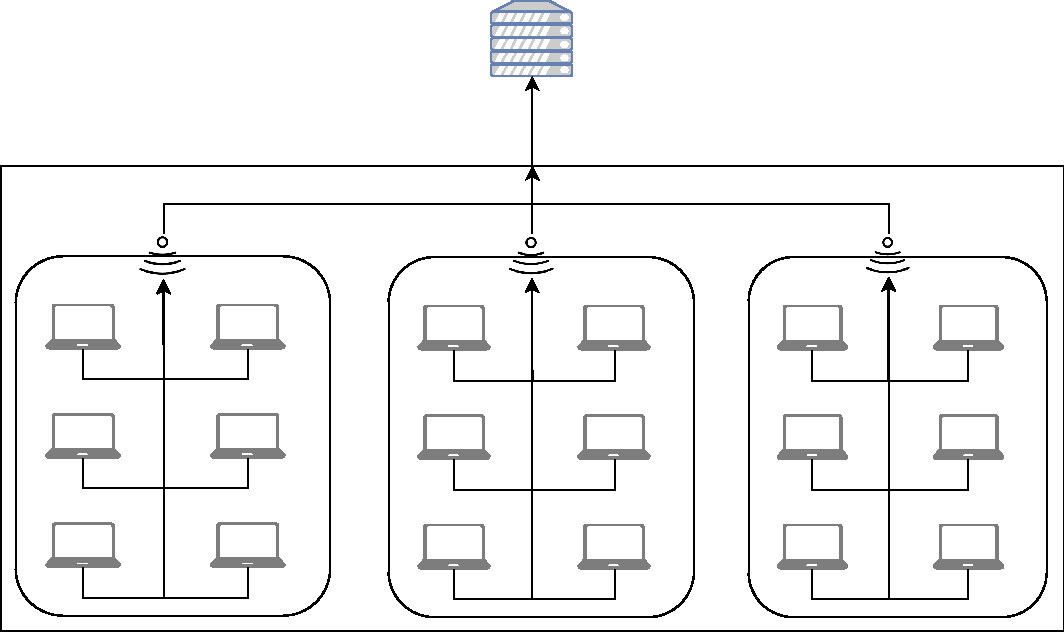
\includegraphics[width=0.8\textwidth]{figures/network_current}
	\caption[A Figure Short-Title]{Netzwerkverkehr in einem herkömmlichen Netzwerk}
	\label{fig:school}
\end{figure}

In den Betrachteten Anwendungsfällen besteht eine hohe zeitlich und inhaltliche Lokalität der Daten. Dies kann genutzt werden um die benötigte Bandbreite zu reduzieren. Dazu soll im Folgenden eine interne Verteilung mittels eines hybriden \pTp Ansatzes untersucht werden. Abbildung \ref{fig:mesh} zeigt exemplarisch den Aufbau eines solchen Netzwerkes. Anstatt das jeder Client sich die Ressource von einem externen Server lädt, lädt nur noch ein Nutzer je Subnetz die Resource über das WAN. Dieser verteilt die Resource dann im internen Netzwerk an andere Clients die diese dann ebenfalls wieder bereitstellen.

Benötigt ein Client eine Resource versucht er zuerst die Resource über sein \pTp Mesh zu laden. Ist dies nicht möglich lädt er sie über einen externen Server. Hat ein Peer eine Resource geladen speichert er sie zwischen und stellt sie für andere Clients bereit.

\begin{figure}[!h]
	\centering
	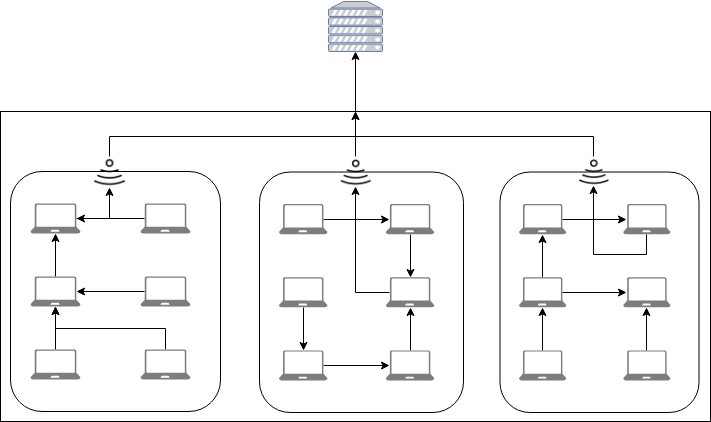
\includegraphics[width=0.8\textwidth]{figures/network_p2p}
	\caption[A Figure Short-Title]{Netzwerkverkehr in einem Peer To Peer CDN}
	\label{fig:mesh}
\end{figure}

Da sowohl im Kontext der Schule als auch bei Unternehmen kein Wissen im Bereich der Computer Administration seitens der Nutzer vorausgesetzt werden kann, wurde ein Ansatz gewählt werden der keine Installation auf Seiten der Nutzer benötigt. Das Nutzererlebnis soll dabei nicht negativ beeinflusst werden. 

% herausstellen das ein plugin entwickelt wird das eingebunden werden kann


% schon geschrieben:
%Genereller Architektur Ansatz
% interne verteilung in subnetzen vs wan verbindung
% Klassische Server architekur mit client und server beschreiben + bild
% p2p mit bild zeigen netzarchitektur
% kommunikation zwischen peer anhand von vereinfachter architektur beschreiben
%	bild peer to peer zwischen browsern ohne service worker
%	peer to peer zwischen browsern
% hybrid p2p CDN ansatz
% keine installation auf clientseite
% domainen wissen soll genutzt werden um clients zu verbinden
% 
%
%
%


%bild schule wie in blockpost?
%
%
%%

% "hybrid p2p cdn"
%konfiguration von subnetzen?
\section{Netzwerk Strukturen}
\todo{Anwendungsfall analyse? -- evt in einleitung schieben.}

Im Folgenden wird betrachtet wie die Netzwerkstruktur der Clients im Falle von Slidesync und \schulCloud zusammensetzen.
\subsection{\schulCloud}
Bei der \schulCloud lassen sich im wesentlichen zwei Hauptanwendungsszenarien unterscheiden. Zum einen die Anwendung im Unterricht. Der Lehrer stellt z.B. eine Aufgabe die mit Hilfe der \schulCloud durchgeführt werden soll. Daraufhin besuchen die Schüler die entsprechende Seite und bearbeiten die Aufgabe. In einem kurzen Zeitfenster laden also mehrer Schüler während sie sich im gleichen lokalen Netzwerk befinden, dem der Schule, die selben Inhalte herunter. Bei dem anderen Szenario wird die \schulCloud außerhalb des Unterrichts genutzt. Z.B. bereitet der Lehrer den Unterricht vor oder die Schüler bearbeiten gestellte Hausaufgaben. Die Nutzer befinden sich nicht zwangsläufig im selben Netzwerk. Auch Laden die Nutzer die selben Daten nicht notwendigerweise in einem kurz Zeitfenster sondern verteilt über einen längeren Zeitraum. Es findet jedoch auch keine so starke Auslastung des Netzwerks statt. Deshalb wird im Rahmen dieser Arbeit vor allem das erste Szenario betrachtet.

\subsection{Slidesync}
Die Verteilung der Clients auf Netzwerke kann sich bei Slidesync von Event zu Event stark unterscheiden. Da sich Slidesync jedoch hauptsaächlich für Streams von mittleren bis großen Unternehmen wendet, lässt sich beobachten das viele der Nutzer sich gemeinsam in einem lokalen Netzwerk, einem Standort, befinden. Um die Last der Unternehmensnetzwerke zu reduzieren, werden bei einigen Unternehmen caching Server eingesetzt. Betrachtet man 10 Events mit caching Infrastruktur im Internen netz stellt man fest das 64\% der Teilnehmer aus dem internen Netz auf das Event zugegriffen haben. In dieser Arbeit wird betrachtet wie die Last auf das interne Netz reduziert werden kann ohne das zusätzliche caching Server eingesetzt werden müssen.

\subsection{Gemeinsamkeiten}

\section{Architektur}
\begin{figure}[!h]
	\centering
	\includegraphics[width=0.8\textwidth]{figures/service_worker_app}
	\caption[A Figure Short-Title]{Service Worker - Webrtc}
	\label{fig:mesh}
\end{figure}

\begin{itemize}
	\item Browser based without plugin
	\item Service Worker -- > WEBRTC
	\item Script für execution
	\item Webrtc - Datachannel
	\item Service worker cached request
	\item warum service worker
	\item 	vergleich anderer Ansätze
	\item 	Literatur anschauen
\end{itemize}
%Für unsere Implementation wird für das Zwischenspeichern von Daten ein Serviceworker eingesetzt. Serviceworker können wie ein Proxy zwischen dem Webbrowser und dem Webserver agieren, welcher die Webseite bereitstellt. Stellt ein Browser eine Anfrage, so wird diese vom Serviceworker abgefangen. Der Serviceworker schaut zunächst in seinem Cache, der sog. IndexDB, ob er die gestellte Anfrage beantworten kann. Ist dies nicht der Fall, so wird die Anfrage an den Webserver weitergeleitet. Wird die gleiche Anfrage nochmals gestellt, kann diese aus dem Cache beantwortet werden, da gestellte Anfragen eine gewisse Zeit lang zwischengespeichert werden.
%\begin{figure}[!h]
%	\centering
%	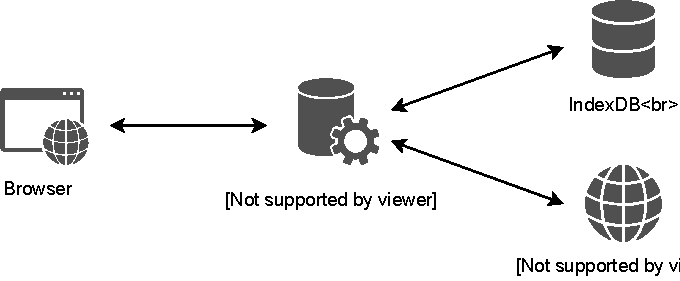
\includegraphics[width=0.8\textwidth]{figures/ServiceWorker}
%	\caption[A Figure Short-Title]{A Figure Title}
%	\label{fig:sequenceDiagram}
%\end{figure}
%
%
%Die von uns eingesetzte Technologie zur Übertragung von Daten zwischen Browsern ist WebRTC. WebRTC ist ein offener Standard und ermöglicht es Browser paarweise zwecks Datenaustausch zu verbinden. Der große Vorteil dieser Technologie ist, dass sie direkt von modernen Browsern unterstützt wird, wodurch keine zusätzliche Software installiert werden muss. Konkret wird von uns ein sog. DataChannel genutzt.
%
%Für den Datenaustausch müssen wechselseitig DataChannel zueinander aufgebaut werden. Die Ausgangslage ist, dass die Schüler wissen, dass es den anderen gibt, aber nicht wie der jeweils andere zu erreichen ist. Um diese Problematik zu lösen, existiert ein Vermittlungsserver (Signaling server).
%
%Als erstes werden Informationen, über die Verbindung die aufgebaut werden soll, an den Signaling server gesendet. Technisch wird ein SDP-offer gesendet, wobei SDP für Session Description Protocol steht. Dieses SDP-offer leitet der Signaling server an die Schüler in der Klasse/Schule weiter. Geantwortet wird mit einer SDP-answere, welche Informationen über die abgestimmte Verbindung enthält und über den Signaling server zurück geleitet wird.
%
%Damit eine direkte Verbindung aufgebaut werden kann, müssen über den Signaling server noch weitere Informationen wie ICE-Kandidaten ausgetauscht werden. ICE steht hierbei für Interactive Conectivity Establishment und ist fester Bestandteil von WebRTC. Es ist für den Aufbau der Browser-zu-Browser-Verbindung verantwortlich. ICE-Kandidaten enthalten hauptsächlich Informationen darüber wie ein bestimmter Nutzer erreichbar ist (also z.B. private oder öffentliche IP-Adresse). Ermittelt werden diese ICE-Kandidaten mithilfe eines STUN-Servers und dem dazugehörigen Session Traversal Utilities for NAT (STUN) Protokoll. Wie der Name des Protokolls schon verrät, wird es vor allem benötigt um auch Nutzer erreichen zu können die keine eigene öffentliche IP-Adresse besitzen, bei denen also Network address translation (NAT) eingesetzt wird. Dies ist aufgrund der mangelnden Anzahl an IPv4-Adressen bei fast jedem Internetnutzer der Fall.
%
%In dem Signaling server selbst wird die Logik abgebildet, wie die Klassen und Schüler miteinander in Verbindung stehen. Implementiert wurde dieser mit socket.io, da die native Klassenorganisation und Websocket-Technologie sich nahezu perfekt für unser Szenario anbot.

\section{Mesh Zuordnung - Verbinden von Peers}
Im Folgenden werden verschiedene Zuordnungsstragien zur Bildung von Peer Meshes diskutiert. Dazu wird der typische Workload beider Anwendungen analysiert um eine jeweils geeignete Strategie zu wählen. 

- Vergleich von Meshing verfahren/peer routing aus literatur
\subsection{Routing}
-Datenstruktur
- Dezentralisierte Datenspeicherung
- Daten werden über SPeicherknoten verteilt
- Jeder Knoten eintrag in Hashtabelle
- direct storage: Daten in Hashtabelle
	- nur für kleine Daten
- indirect storage: Verweis auf daten in Hashtabelle

Eigenschaften:
Fehlertoleranz
Lastenverteilung
Robustheit
Selbstorganisation
Skalierbarkeit


consistent hashing
- Server zum routen
https://www.coralcdn.org/pubs/
\subsubsection{Chord}

How to save files in advance???
save file references
\subsubsection{Kademlia}
\subsubsection{IPFS}
\subsubsection{Kelips}
\subsubsection{Pastry}
\subsection{\schulCloud}
Analyse workload mit grafik

Schulcloud
- Global
einfache umsetzung
Kurs unabhänige assets können geteilt werden
Maximale Mesh größe
Mehrere Meshes nötig
Möglicherweise nicht im Mesh mit relevanten Peers
Maximiert die Anzahl der Peers pro Mesh
Wahrscheinlichkeit für selbes Subnetz eher gering
Funktioniert auch mit wenigen Clients
Ineffektiv wenn viele Clients vorhanden sind

- Schule
Einfache Umsetzung
Funktioniert auch mit wenigen Clients
Relativ hohe trefferrate da schulen selten mehr als 1000 Schüler hat
Max mesh größe um die 256(Chrome)
Relativ wahrscheinlich gleiches Subnetz

- Kurs
Hohe trefferrate
Kleine Meshes
benötigt mehr Clients
Relativ wahrscheinlich gleiches Subnetz --> Daten die das bestätigen

hybride Ansätze:
Zwei priorisierte Meshes Schule und Klasse

Berechnung eines Scores für jeden Peer:
Möglichst viele gemeinsame kurse
Liste von Kursen für jeden Peer
Schnittmenge für jeden peer der online ist bilden
Kardinalität der Menge = Score von Peer
Rechenaufwendig Aber machbar
Beste Trefferrate
Funktioniert wenn wenige und wenn viele Peers anwesend sind

\subsection{Slidesync}
Slidesync ist eine Plattform deren Nutzung stark durch die durchgeführten live Events dominiert wird. Ein Moderator erstellt das Event lädt die notwendigen Assets, z.B. Foliensätze, hoch. Live Events werden für eine bestimmte Zeit festgesetzt und Teilnehmer laden zum start des Events die Seite.\todo{Grafik visits} Ein Großteil des entstandenen Traffics besteht aus HLS Videoseqmenten. Jeder Teilnehmer eines Events benötigt die selben Inhalte.\todo{Grafik traffic} 

Die Peer Meshes in Slidesync werden als voll vermaschte Netzte abgebildet. Da alle Teilnehmer eines Events zu großen Teilen die selben Daten benötigen können sie in dem selben Mesh untergebracht werden. Um zu gewährleisten das sich die Peers im Selben Subnetz befinden teilen sich nur solche ein Peer Mesh die sich in der Selben IP Range befinden. Ein weiterer wichtiger Factor ist der Kommunkationsoverhead der durch das halten von Verbindungen zu vielen Peers entsteht. Deshalb ist es nicht möglich bei größeren Events alle Peers im selben Peer Mesh unter zu bringen. Deshalb werden Sub Meshes gebildet in denen sich eine maximale Anzahl an Peers befinden können. 

Abbildung \ref{fig:mesh-slidesync} zeigt eine beispielhafte Aufteilung von Peer Meshes für ein Event. Für Netzwerk A und B werden jeweils zwei Meshes erzeugt und nur solche Clients werden miteinander verbunden die sich auch im Selben Subnetz befinden. Jedes Netzwerk wird wiederum in zwei Sub-Meshes unterteilt.

\begin{figure}[!h]
	\centering
	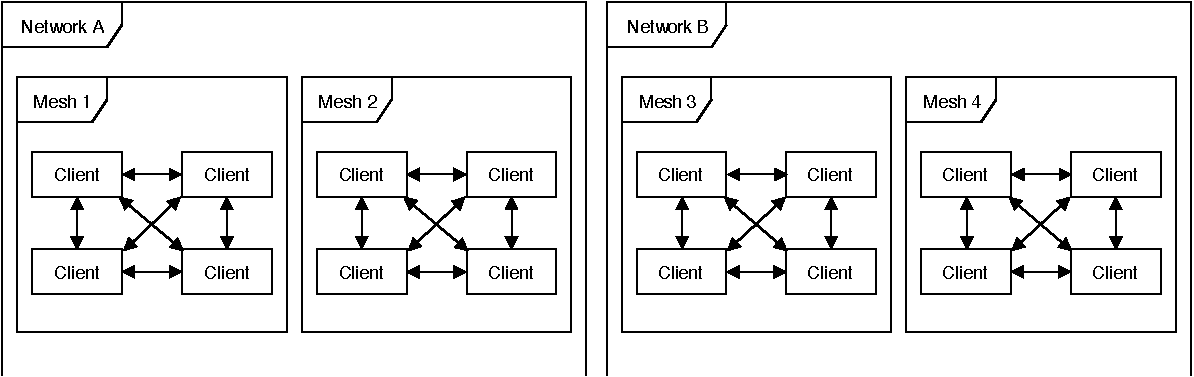
\includegraphics[width=0.8\textwidth]{figures/slidesync_peer_meshes}
	\caption[A Figure Short-Title]{Peer to Peer Meshes - Slidesync}
	\label{fig:mesh-slidesync}
\end{figure}


%Analyse workload
%
%Live Streaming
%- Event basiert
%- interessante Inhalte zum Teilen: Video stream
%- Viele Nutzer pro Event seite
%- aufsplittung von Peers anhand von lokalen Netzwerken wenn verfügbar

% voll vermaschtes netz
% mit bild
% Nutzung des anwendungswissens
% ip subnetz plus gleicher Kurs/stream


\section{Routing - finden von Ressourcen}

Um das \pTp Netzwerk als \cdn Nutzbar zu machen ist es wichtig das ein Peer in der Lage ist herauszufinden wer welche resource bereitstellt. Dazu lassen sich verschiedene Ansätze verfolgen.

DHT\todo{distributed hash tables erklären}

Structured vs untructured

Da das Routing von Ressourcen bei den Betrachteten Anwendungsfällen in einem Zeitkritischen Moment erfolgen muss wurde sich für einen anderen Ansatz entschieden. Jeder Peer hält eine Hashtabelle mit den Ressourcen seiner Peers vor. Fügt ein Peer eine neue Ressource zu seinem Cache hinzu oder entfernt sie muss er alle verbundenen Peers über diese Änderung informieren. Dadurch muss im Falle einer Anfrage nicht erst die Ressource im Netzwerk gesucht werden. Dies ist möglich durch die Struktur des Netzwerkes. Da nicht alle Peers miteinander verbunden sind sondern voll vermaschte sub-meshes gebildet werden ist es möglich alle relevanten Peers über Änderungen zu informieren. Dadurch ist es möglich die Rechenleistung für das auffinden von Ressourcen in einen weniger Zeitkritischen Moment zu verlagern. Jedoch hat dies zur Folge das die Meshes so gebildet werden müssen das die Peers möglichst viele Ressourcen gemeinsam benötigen. Ist eine Ressource nicht im Mesh vorhanden kann sie vom Server geladen werden. 


%Structured vs unstructured networks
%
%Kollaborative File Sharing Protokolle wie z.B. Bitorrent verwenden häufig verteilte Hashtabellen zum auffinden von Ressourcen im Netzwerk. 
%Zhang proposed a DHT based P2P resource pool, SOMO
%[22], [23] to manage global resources and optimize multiple
%ALM (Application Layer Multicast) sessions,

%server hält liste vor --> kommunikation mit server nötig. \study
%
%peer fragt im Netzwerk an --> mehr kommunikation wenn in zeitkritischem moment \study
%
%peer halten liste von requests aktuell. Kommunikationsoverhead in zeitunkritischem moment \study
%	 peer weiß immer bei wer welche resource hat

% evtl diskussion verschiedener methoden 
%   server hält liste vor --> kommunikation mit server nötig
% peer fragt im Netzwerk an --> mehr kommunikation wenn in zeitkritischem moment
% peer halten liste von requests aktuell
%    kommunikationsoverhead in zeitunkritischem moment
%	 peer weiß immer bei wer welche resource hat
% am Anfang wird die zuordnung von einem peer an den neuen geschickt

\subsection{ Updates }
\subsection{Subnetzerkennung}
\subsection{ Struktur von IP Adressen}
eher Konzept


\section{Wiederverwendbarkeit}
%Plug and play
%Konfigurierbarkeit
%einfaches einbinden in existierende anwendungen über npm
%javascript modul
%support von eigenen oder öffentlichen stun servern
%%Plug and play
\section{Open Source}
%was ist open source
%bereitstellung für die öffentlichkeit
%
